\section{Introduction}
\label{sec:introduction}

The discovery of a Higgs ($\PHiggs$) boson by the ATLAS and CMS experiments~\cite{Higgs-Discovery_ATLAS,Higgs-Discovery_CMS}
represents a major step towards our understanding of electroweak symmetry breaking (EWSB),
as well as of the mechanism that generates the masses of quarks and leptons, 
the particles that constitute the `` ordinary'' matter in our universe.
In a combined analysis of the data recorded by ATLAS and CMS during LHC Run $1$, 
the mass of the $\PHiggs$ boson has been measured to be $125.09 \pm 0.24$~\GeV~\cite{HIG-14-042}.
Recent analyses of data collected during LHC Run $2$ corroborate this value~\cite{ATLAS:2020coj,CMS:2020xrn}.
The Standard Model (SM) of particle physics makes precise predictions for all properties of the $\PHiggs$ boson, given its mass. 
The predictions have been probed by measurements of its spin and CP quantum numbers~\cite{HIG-14-018,Aad:2015mxa,ATLAS:2020evk,CMS:2021nnc},
of its couplings to gauge bosons and to down-type fermions~\cite{HIG-15-002},
and of its total decay width, including decays to invisible particles~\cite{CMS:2018yfx,CMS:2019ekd,Aad:2015pla,ATLAS:2018jym}.
So far, all measured properties of the discovered particle are consistent with the expectation for a SM $\PHiggs$ boson 
within the uncertainties of these measurements.
Evidence for its coupling to up-type fermions, at a strength compatible with the SM expectation, has been observed recently~\cite{Aaboud:2018urx,HIG-17-035}.

The SM predicts $\PHiggs$ boson self-interactions via trilinear and quartic couplings. 
Measurements of the $\PHiggs$ boson self-interactions will allow to determine the potential of the Higgs field,
thereby ultimately either confirming or falsifying that the Brout-Englert-Higgs mechanism of the SM is responsible for EWSB.
The measurement of the quartic coupling is not possible at the LHC~\cite{deFlorian:2019app}, 
even with the $3000$~fb$^{-1}$ of data foreseen to be recorded at $\sqrt{s}=14$~\TeV center-of-mass energy during the upcoming HL-LHC data-taking period~\cite{HL-LHC-TDR},
as the cross section of the corresponding process, triple $\PHiggs$ boson production, is much too small, 
on the level of $5 \cdot 10^{-2}$~\fb~\cite{Plehn:2005nk,Binoth:2006ym}.

The trilinear coupling ($\lambdaHHH$) can be determined at the LHC, by measuring the rate for $\PHiggs$ boson pair production ($\dihiggs$). 
In analogy to the production of single $\PHiggs$ bosons, 
four different processes are relevant for $\dihiggs$ production at the LHC: 
gluon fusion ($\ggHH$), vector boson fusion ($\qqHH$), the associated production with a $\PW$ or $\PZ$ boson ($\VHH$),
and associated production of the $\PHiggs$ boson pair with a pair of top quarks ($\ttHH$).
The total $\dihiggs$ production rate is dominated by the $\ggHH$ process.
Its cross section has been computed at next-to-next-to-leading order (NNLO) in perturbative quantum chromodynamics (pQCD),
with resummation of soft gluon contributions at next-to-next-to-leading logarithmic accuracy.
Including corrections for finite top quark mass effects, computed at next-to-leading order (NLO),
the SM cross section for the $\ggHH$ process amounts to $31.05^{+1.40}_{-1.98}$~\fb at $\sqrt{s} = 13$~\TeV center-of-mass energy~\cite{Grazzini:2018hh}.
The cross section is rather small, as the production of $\PHiggs$ boson pairs through gluon fusion is a loop induced process,
and is further reduced by the negative interference of two competing production mechanisms.
The leading order (LO) Feynman diagrams for the two competing production mechanisms are shown in Fig.~\ref{fig:ggHH_FeynmanDiagram}.
The right diagram, referred to as the ``box'' diagram, does actually not depend on the trilinear $\PHiggs$ boson self-coupling $\lambdaHHH$.
The diagram that provides the sensitivity to $\lambdaHHH$ is the ``triangle'' diagram shown on the left.
Both diagrams depend on the coupling of the $\PHiggs$ boson to the top quark, denoted by the symbol $\yt$,
which is measured with an uncertainty of order $10\%$ at present~\cite{Aaboud:2018urx,HIG-17-035}.
The cross sections for the $\qqHH$, $\VHH$, and $\ttHH$ process are more than one order of magnitude smaller~\cite{Baglio:2012np}.
As the sensitivity of experimental analyses at the LHC is limited by the small signal rate at present,
we will focus on the $\ggHH$ production process in this paper.

\begin{figure}
\setlength{\unitlength}{1mm}
\begin{center}
\begin{tabular}{ccc}
\raisebox{-.45\height}{\resizebox{0.43\textwidth}{!}{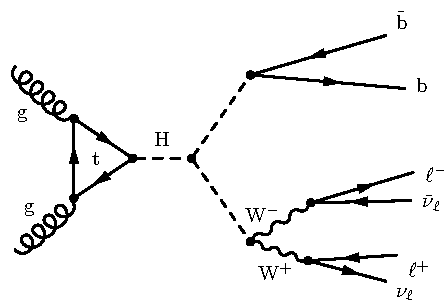
\includegraphics[bb=0 0 214 147]{figures/hh_triangle.pdf}}} &
\qquad + &
\raisebox{-.45\height}{\resizebox{0.43\textwidth}{!}{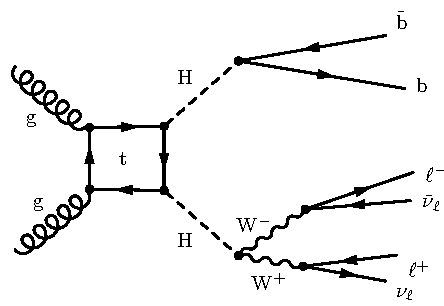
\includegraphics[bb=0 0 214 147]{figures/hh_box.pdf}}}
\end{tabular}
\end{center}
\caption{
  Leading order (LO) Feynman diagrams for the $\ggHH$ production process in $\Pp\Pp$ collisions at the LHC,
  with subsequent decay of the $\PHiggs$ boson pair via $\PHiggs\PHiggs \to \Pbottom\APbottom\PW\PW\virt \to \Pbottom\APbottom \, \ellPlusnu\ellMinusnu$.
  The asterisk ($\virt$) denotes an off-shell $\PW$ boson.
}
\label{fig:ggHH_FeynmanDiagram}
\end{figure}

The $\dihiggs$ production rate may be enhanced significantly in case an as yet unknown resonance decays to pairs of $\PHiggs$ bosons.
Such resonances are predicted in models with two Higgs doublets~\cite{Craig:2013hca,Nhung:2013lpa}, composite $\PHiggs$ boson models~\cite{Grober:2010yv,Contino:2010mh}, 
Higgs portal models~\cite{Englert:2011yb,No:2013wsa}, and models involving extra dimensions~\cite{Randall:1999ee}.
In the absence of new resonances decaying into $\PHiggs$ boson pairs,
the $\dihiggs$ production cross section may be enhanced by deviations of the couplings $\lambdaHHH$ and $\yt$ from the SM expectation for these couplings
and by the contribution of new particles to the loops 
that are present in the triangle and box diagrams shown in Fig.~\ref{fig:ggHH_FeynmanDiagram}.
%The effect of contributions from new particles to these loops can adequately be described by anomalous $\PHiggs$ boson couplings.
%More specifically,
%the production of $\PHiggs$ boson pairs via gluon fusion in Beyond the Standard Model (BSM) theories can be described to leading approximation by the non-linear Lagrangian~\cite{Buchmuller:1985jz}:
%\begin{eqnarray}
%\mathcal{L} & = & \frac{1}{2} \partial_{\mu}\PHiggs\partial^{\mu}\PHiggs - \frac{1}{2} m_{\PHiggs}^{2} \PHiggs^{2} - \kappa_{\lambda} \lambdaHHH^{\textrm{SM}} v \PHiggs^{3} \nonumber \\
% & & \quad -\frac{m_{\Ptop}}{v} \, \left( v + \kappa_{\Ptop} \PHiggs + \frac{c_{2}}{v} \PHiggs\PHiggs \right) \, \left( \bar{\Ptop}_{\textrm{L}} \Ptop_{\textrm{R}} + \textrm{h.c.} \right) 
%+ \frac{1}{4} \frac{\alpha_{\textrm{s}}}{3 \pi v} \, \left( c_{\Pgluon} \PHiggs - \frac{c_{2\Pgluon}}{2 v} \PHiggs\PHiggs \right) \, \textrm{G}^{\mu\nu}\textrm{G}_{\mu\nu} \, ,
%\end{eqnarray}
%where $v = 246$~\GeV denotes the vacuum expectation value of the Higgs field
%and the parameters $\kappa_{\lambda} = \lambdaHHH/\lambdaHHH^{\textrm{SM}}$ and $\kappa_{\Ptop} = \yt/\yt^{\textrm{SM}}$ 
%quantify the deviations of the trilinear $\PHiggs$ boson self-coupling and of the coupling of the $\PHiggs$ boson to the top quark from their SM values.
%Besides the two parameters $\kappa_{\lambda}$ and $\kappa_{\Ptop}$,
%the Lagrangian contains the coefficients of three BSM operators which account for contact interactions 
%between a $\PHiggs$ boson and either one ($c_{\Pgluon}$) or two ($c_{2\Pgluon}$) gluons
%and between a pair of $\PHiggs$ bosons and a pair of top quarks ($c_{2}$).
%The contact interactions can be interpreted in an effective field theory (EFT) approach~\cite{Buchalla:2015wfa, Goertz:2014qta}.
The effect of contributions from new particles to these loops can adequately be described by anomalous $\PHiggs$ boson couplings
in an effective field theory (EFT) approach~\cite{Buchalla:2015wfa, Goertz:2014qta}.
The production of $\PHiggs$ boson pairs in the absence of new resonances is referred to as non-resonant $\dihiggs$ production,
the case that we focus on in this paper.

%The distribution in mass of the $\PHiggs$ boson pair, $m_{\dihiggs}$, is rather broad in this case.
%Deviations of the $\PHiggs$ boson couplings from their SM values
%induces different interference patterns between the triangle and box diagrams.
%Besides affecting the $\dihiggs$ production cross section,
%the change in interference patterns may  significantly alter the distribution in $m_{\dihiggs}$
%and the distributions in the momenta and angles of the particles reconstructed in the final state.

The ATLAS and CMS collaborations have searched for non-resonant $\dihiggs$ production in the decay channels 
$\dihiggs \to \Pbottom\APbottom\Pbottom\APbottom$, $\Pbottom\APbottom\Pgt\Pgt$, $\Pbottom\APbottom\PW\PW\virt$, $\Pbottom\APbottom\Pgamma\Pgamma$
using the data recorded during LHC Runs $1$ and $2$~\cite{HIG-13-032,HIG-15-013,HIG-17-006,HIG-17-030,Sirunyan:2020xok,Aad:2015xja,Aaboud:2018knk,Aaboud:2018ftw,Aaboud:2018sfw,Aaboud:2018zhh}.
ATLAS has further performed searches in the decay channels $\dihiggs \to \Pgamma\Pgamma\PW\PW\virt$ and $\PW\PW\virt\PW\PW\virt$~\cite{Aad:2015xja,Aaboud:2018ewm,Aaboud:2018ksn}.
The asterisk ($\virt$) denotes $\PW$ bosons that are off-shell.
Phenomenological studies of non-resonant $\dihiggs$ production are presented in 
Refs.~\cite{Baur:2002rb,Baur:2002qd,Baur:2003gpa,Baur:2003gp,Dolan:2012rv,Papaefstathiou:2012qe,Baglio:2012np,deLima:2014dta,Wardrope:2014kya,Behr:2015oqq,Li:2015yia,Adhikary:2017jtu}.
No evidence for a signal has been found in the LHC data so far.
The present analyses are able to probe the existence of a SM-like $\dihiggs$ signal produced with a cross section of order $10$ times the SM production rate.

The decay channel providing the highest sensitivity for an SM-like $\dihiggs$ signal 
is the $\Pbottom\APbottom\Pgt\Pgt$ channel in case of ATLAS~\cite{Aaboud:2018sfw} and the $\Pbottom\APbottom\Pgamma\Pgamma$ channel in case of CMS~\cite{Sirunyan:2020xok}.
Both channels provide a favorable signal-to-background ratio and are limited mainly by statistical uncertainties at present,
resulting from the limited amount of data that has been recorded so far compared to the small SM $\ggHH$ production cross section.
The channels $\Pbottom\APbottom\Pbottom\APbottom$ and $\Pbottom\APbottom\PW\PW\virt$ provide a significantly larger signal rate,
but suffer from sizeable backgrounds,
arising from QCD multijet production in case of the $\Pbottom\APbottom\Pbottom\APbottom$ channel 
and from top quark pair ($\ttbar$) production in case of the $\Pbottom\APbottom\PW\PW\virt$ channel.
In this paper, we focus on the $\Pbottom\APbottom\PW\PW\virt$ channel,
and in particular on events in which both $\PW$ bosons decay to charged leptons (electrons or muons).
The latter are denoted by the symbol $\Plepton$.
 
\begin{figure}
\setlength{\unitlength}{1mm}
\begin{center}
\begin{tabular}{ccc}
\raisebox{-.45\height}{\resizebox{0.4\textwidth}{!}{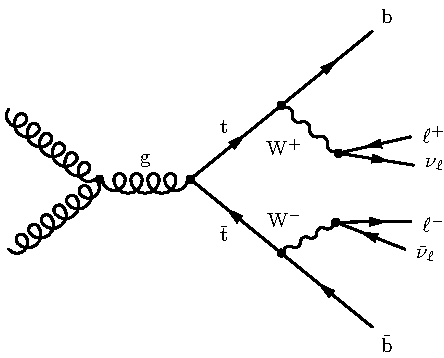
\includegraphics[bb=0 0 214 172]{figures/ttbar_tri.pdf}}} &
\qquad + &
\raisebox{-.45\height}{\resizebox{0.4\textwidth}{!}{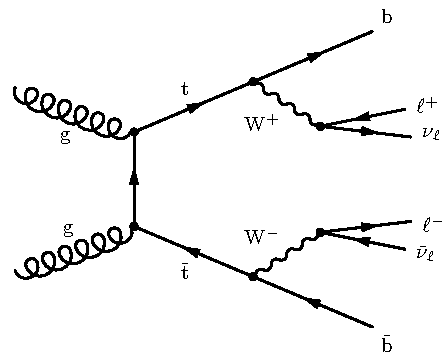
\includegraphics[bb=0 0 214 172]{figures/ttbar.pdf}}}
\end{tabular}
\end{center}
\caption{
  LO Feynman diagrams for $\ttbar$ production in $\Pp\Pp$ collisions at the LHC,
  with subsequent decay of the top quark pair via $\ttbar \to \Pbottom\PW\APbottom\PW \to \Pbottom\ellPlusnu \, \APbottom\ellMinusnu$.
}
\label{fig:ttbar_FeynmanDiagram}
\end{figure}

The separation of the $\dihiggs$ signal from the large $\ttbar$ background constitutes the main experimental challenge in the $\Pbottom\APbottom\PW\PW\virt$ channel.
For a top quark mass of $m_{\Ptop} = 172.8$~\GeV~\cite{PDG},
the cross section for $\ttbar$ production amounts to $825.9^{+46.1}_{-50.5}$~\pb at $\sqrt{s} = 13$~\TeV center-of-mass energy~\cite{Czakon:2011xx}.
The $\ttbar$ background is irreducible in this channel, as it produces the exact same multiplicity of charged leptons, neutrinos, and $\Pbottom$-jets as the $\dihiggs$ signal.
The LO Feynman diagrams for $\ttbar$ production are shown in Fig.~\ref{fig:ttbar_FeynmanDiagram}.
The main handle to separate the $\dihiggs$ signal from the $\ttbar$ background is the difference in event kinematics,
that is, the differences in the distributions of energies and angles of the charged leptons, $\Pbottom$-jets, and of the missing transverse momentum reconstructed in the event.

The present CMS analysis~\cite{HIG-17-006} utilizes machine-learning methods, based on a Deep Neural Network~\cite{ANN,chollet2015keras},
to separate the $\dihiggs$ signal from the $\ttbar$ background, while the current ATLAS analysis~\cite{Aaboud:2018zhh} employs a sequence of hard cuts for this purpose.
In this paper, we propose an alternative multivariate method for the separation of the $\dihiggs$ signal from the $\ttbar$ background,
the matrix element method (MEM)~\cite{Kondo:1988yd,Kondo:1991dw}.

The paper is structured as follows:
In Section~\ref{sec:mem} we describe the MEM and its application to the $\Pbottom\APbottom\PW\PW\virt$ channel.
The application of the MEM requires the computation of multi-dimensional integrals.
The integration is performed numerically and demands a significant amount of computing time, in the order of a few seconds per event.
In order to make the integrals suitable for numeric integration, analytic transformations need to be performed.
The most relevant of these transformations will be described in Section~\ref{sec:mem} and further details will be given in the appendix.
The performance of the MEM in separating the $\dihiggs$ signal from the $\ttbar$ background is studied in Section~\ref{sec:performance}.
The separation is studied on Monte-Carlo truth and on detector level,
for experimental conditions that are characteristic for the ATLAS and CMS experiments during LHC Run $2$.
The latter are simulated using the $\textsc{DELPHES}$ fast-simulation package~\cite{deFavereau:2013fsa}.
We also study the effect of using matrix elements of leading order when applying the MEM to the $\Pbottom\APbottom\PW\PW\virt$ channel
and estimate the computing time required by the method.
We conclude the paper with a summary in Section~\ref{sec:summary}.
